\documentclass[modern]{aastex631}

\usepackage{amsmath}

% Affiliations
\newcommand{\cca}{Center for Computational Astrophysics, Flatiron Institute, 162 Fifth Avenue, New York, NY 10010, USA}
\newcommand{\sbu}{Department of Physics and Astronomy, Stony Brook University, Stony Brook, NY 11794, USA}
\newcommand{\pa}{Department of Physics and Astronomy, Northwestern University, 2145 Sheridan RD, Evanston, IL 60208, USA}
\newcommand{\ciera}{Center for Interdisciplinary Exploration and Research in Astrophysics (CIERA), Northwestern University, 1800 Sherman Ave, Evanston, IL 60201, USA}

% Editing commands
\newcommand{\todo}[1]{\textcolor{red}{TODO: #1}}

% Generated macros
\newcommand{\dNlogmpeak}{\ensuremath{100^{+44}_{-85}}}
\newcommand{\dNlogmpeakunits}{\ensuremath{\dNlogmpeak \, \mathrm{Gpc}^{-3} \, \mathrm{yr}^{-1}}}
\newcommand{\monepctplgplp}{\ensuremath{3.073^{+0.038}_{-0.053}}}
\newcommand{\monepctplgplpunits}{\ensuremath{\monepctplgplp \, M_\odot}}
\newcommand{\mpeakplgplp}{\ensuremath{9.18^{+0.96}_{-0.94}}}
\newcommand{\mpeakplgplpunits}{\ensuremath{\mpeakplgplp \, M_\odot}}
\newcommand{\alphatwoplgplp}{\ensuremath{-2.9^{+2.6}_{-1.7}}}
\newcommand{\mclow}{2.612}
\newcommand{\mclowunits}{\ensuremath{\mclow \, M_\odot}}\newcommand{\mchigh}{17.41}
\newcommand{\mchighunits}{\ensuremath{\mchigh \, M_\odot}}

% Useful definitions
\newcommand{\dd}{\ensuremath{\mathrm{d}}}

\begin{document}
\title{Hiding Out at the Low End: Gaps and Peaks in the Black-Hole Mass Spectrum \\ Hide and Seek \ldots}

\author[0000-0003-1540-8562]{Will M. Farr}
\email{will.farr@stonybrook.edu}
\email{wfarr@flatironinstitute.org}
\affiliation{\sbu}
\affiliation{\cca}

\author[0000-0001-9236-5469]{Vassiliki Kalogera}
\email{vicky@northwestern.edu}
\affiliation{\pa}
\affiliation{\ciera}

\begin{abstract}
    It is not known whether there is a continum of masses of compact objects
    formed from stellar collapse from the heaviest neutron stars to the lightest
    black holes or whether there is a gap in the mass spectrum between these
    classes of objects.  The presence or absence of a mass gap has implications
    for the supernova mechanism, as well as being a fundamental property of the
    compact object mass function.  In X-ray binaries containing black holes a
    gap is observed, but it is not known whether this is representative of a
    true gap in the mass function or due to selection effects or systematic
    biases in mass estimation.  A small number of black holes have been observed
    with luminous companions in non-interacting orbits, but as yet the sample is
    too small to assess the existence of a gap, and in any case selection
    effects in this sample are hard to quantify \todo{Check this!}.  Binary
    black hole mergers detected from gravitational waves in the GWTC-3 transient
    catalog furnish a large sample of several tens of low-mass black holes with
    a well-understood selection function.  Here we analyze the \nevts{} GWTC-3
    merger events with at least one black hole ($3 \, M_\odot < m_1$) and chirp
    masses below those of a $20\,M_\odot$--$20\,M_\odot$ merger ($M_c <
    \mchighunits$) to uncover the structure of the low-mass black hole mass
    function in these systems.  Using flexible parameterized models for the mass
    function, we find a sharp peak in the mass function at $m =
    \mpeakplgplpunits$, associated with merger rates $m_1 m_2 \mathrm{d} N /
    \mathrm{d} m_1 \mathrm{d} m_2 \mathrm{d} V \mathrm{d} t = \dNlogmpeakunits$.
    The mass function falls by about an order of magnitude both below and above
    this peak.  Toward the lowest masses, the mass function may or may not
    flatten; we find that the $1\%$ black hole mass in our most flexible model
    is $m_{1\%} = \monepctplgplpunits$. In other words, this sample of low-mass
    black holes does not require a mass gap but may permit one; observations in
    the currently-ongoing ``O4'' observation run should distinguish these
    possibilities.  Toward higher masses, the mass function declines steeply,
    with power law slopes $\mathrm{d} N / \mathrm{d} m \sim m^{\alpha}$, $\alpha
    = \alphatwoplgplp$.  The presence of a peak at $m \sim 9 \, M_\odot$ is
    suggested by several models of stellar evolution.
\end{abstract}

\section{Introduction}

Definition of our mass functions:
\begin{equation}
    \label{eq:intensity-definition}
    m_1 m_2 \frac{\dd N}{\dd m_1 \dd m_2 \dd V \dd t} = R \left(1 + \left(\frac{1}{1 + 1.9}\right)^{5.6} \right) f\left( m_1 \right) f\left( m_2 \right) g(m_1, m_2) \frac{\left( 1 + z \right)^{2.7}}{1 + \left( \frac{1+z}{1+1.9} \right)^{5.6}}
\end{equation}

The ``common'' mass function $f$ takes either a broken power law form,
\begin{equation}
    f(m) = \begin{cases}
        \left( \frac{m}{m_b} \right)^{\alpha_1} & m < m_b \\
        \left( \frac{m}{m_b} \right)^{\alpha_2} & m_b < m
    \end{cases},
\end{equation}
or a sum of a broken power law and a Gaussian,
\begin{equation}
    f(m) = f_g \exp\left( - \frac{\left( m - \mu \right)^2}{2 \sigma^2} \right) + \left( 1 - f_g \right) 
    \begin{cases}
        \left( \frac{m}{\mu} \right)^{\alpha_1} & m < \mu \\
        \left( \frac{m}{\mu} \right)^{\alpha_2} & \mu < m
    \end{cases}.
\end{equation}
The ``pairing function'' \citep{Fishbach2020} $g$ is a power law in the total
mass,
\begin{equation}
    g(m_1, m_2) = \left( \frac{1 + \frac{m_2}{m_1}}{2} \right)^{\beta}.
\end{equation}
With these definitions, $R$ is the merger rate per natural log mass squared, per
comoving volume, per time at redshift $z = 0$, $m_1 = m_2 = \mu, m_b$.  We use
the convention $m_2 \leq m_1$.  The parameter $\alpha_1$ is the power law slope
of the mass function much below the break mass $m_b$ or mean mass $\mu$,
$\alpha_2$ is the power law slope of the mass function much above $m_b$ or
$\mu$.  The parameter $\beta$ is the power law slope of the mass ratio in the
pairing function\footnote{We also explored Gaussian pairing functions,
\begin{equation}
    g\left(m_1, m_2 \right) \propto \exp\left( - \left( m_2/m_1 - \mu_q \right)^2 /
\left( 2 \sigma_q^2 \right) \right);
\end{equation} 
but found no qualitative and few quantitative differences with the results
reported here.}.  The parameter $f_g$ is the fraction of the merger rate at $m_1
= m_2 = \mu$ that is in the Gaussian component of the mass function.  When
normalizing the ``common'' mass function $f$ to be a probability distribution
for $m_\mathrm{low} \leq m \leq m_\mathrm{high}$ we will write 
\begin{equation}
    \label{eq:pm-definition}
    p(m) \equiv \frac{f(m)}{\int_{m_\mathrm{low}}^{m_\mathrm{high}} \dd m' \, f(m')}.
\end{equation}

\begin{figure}
    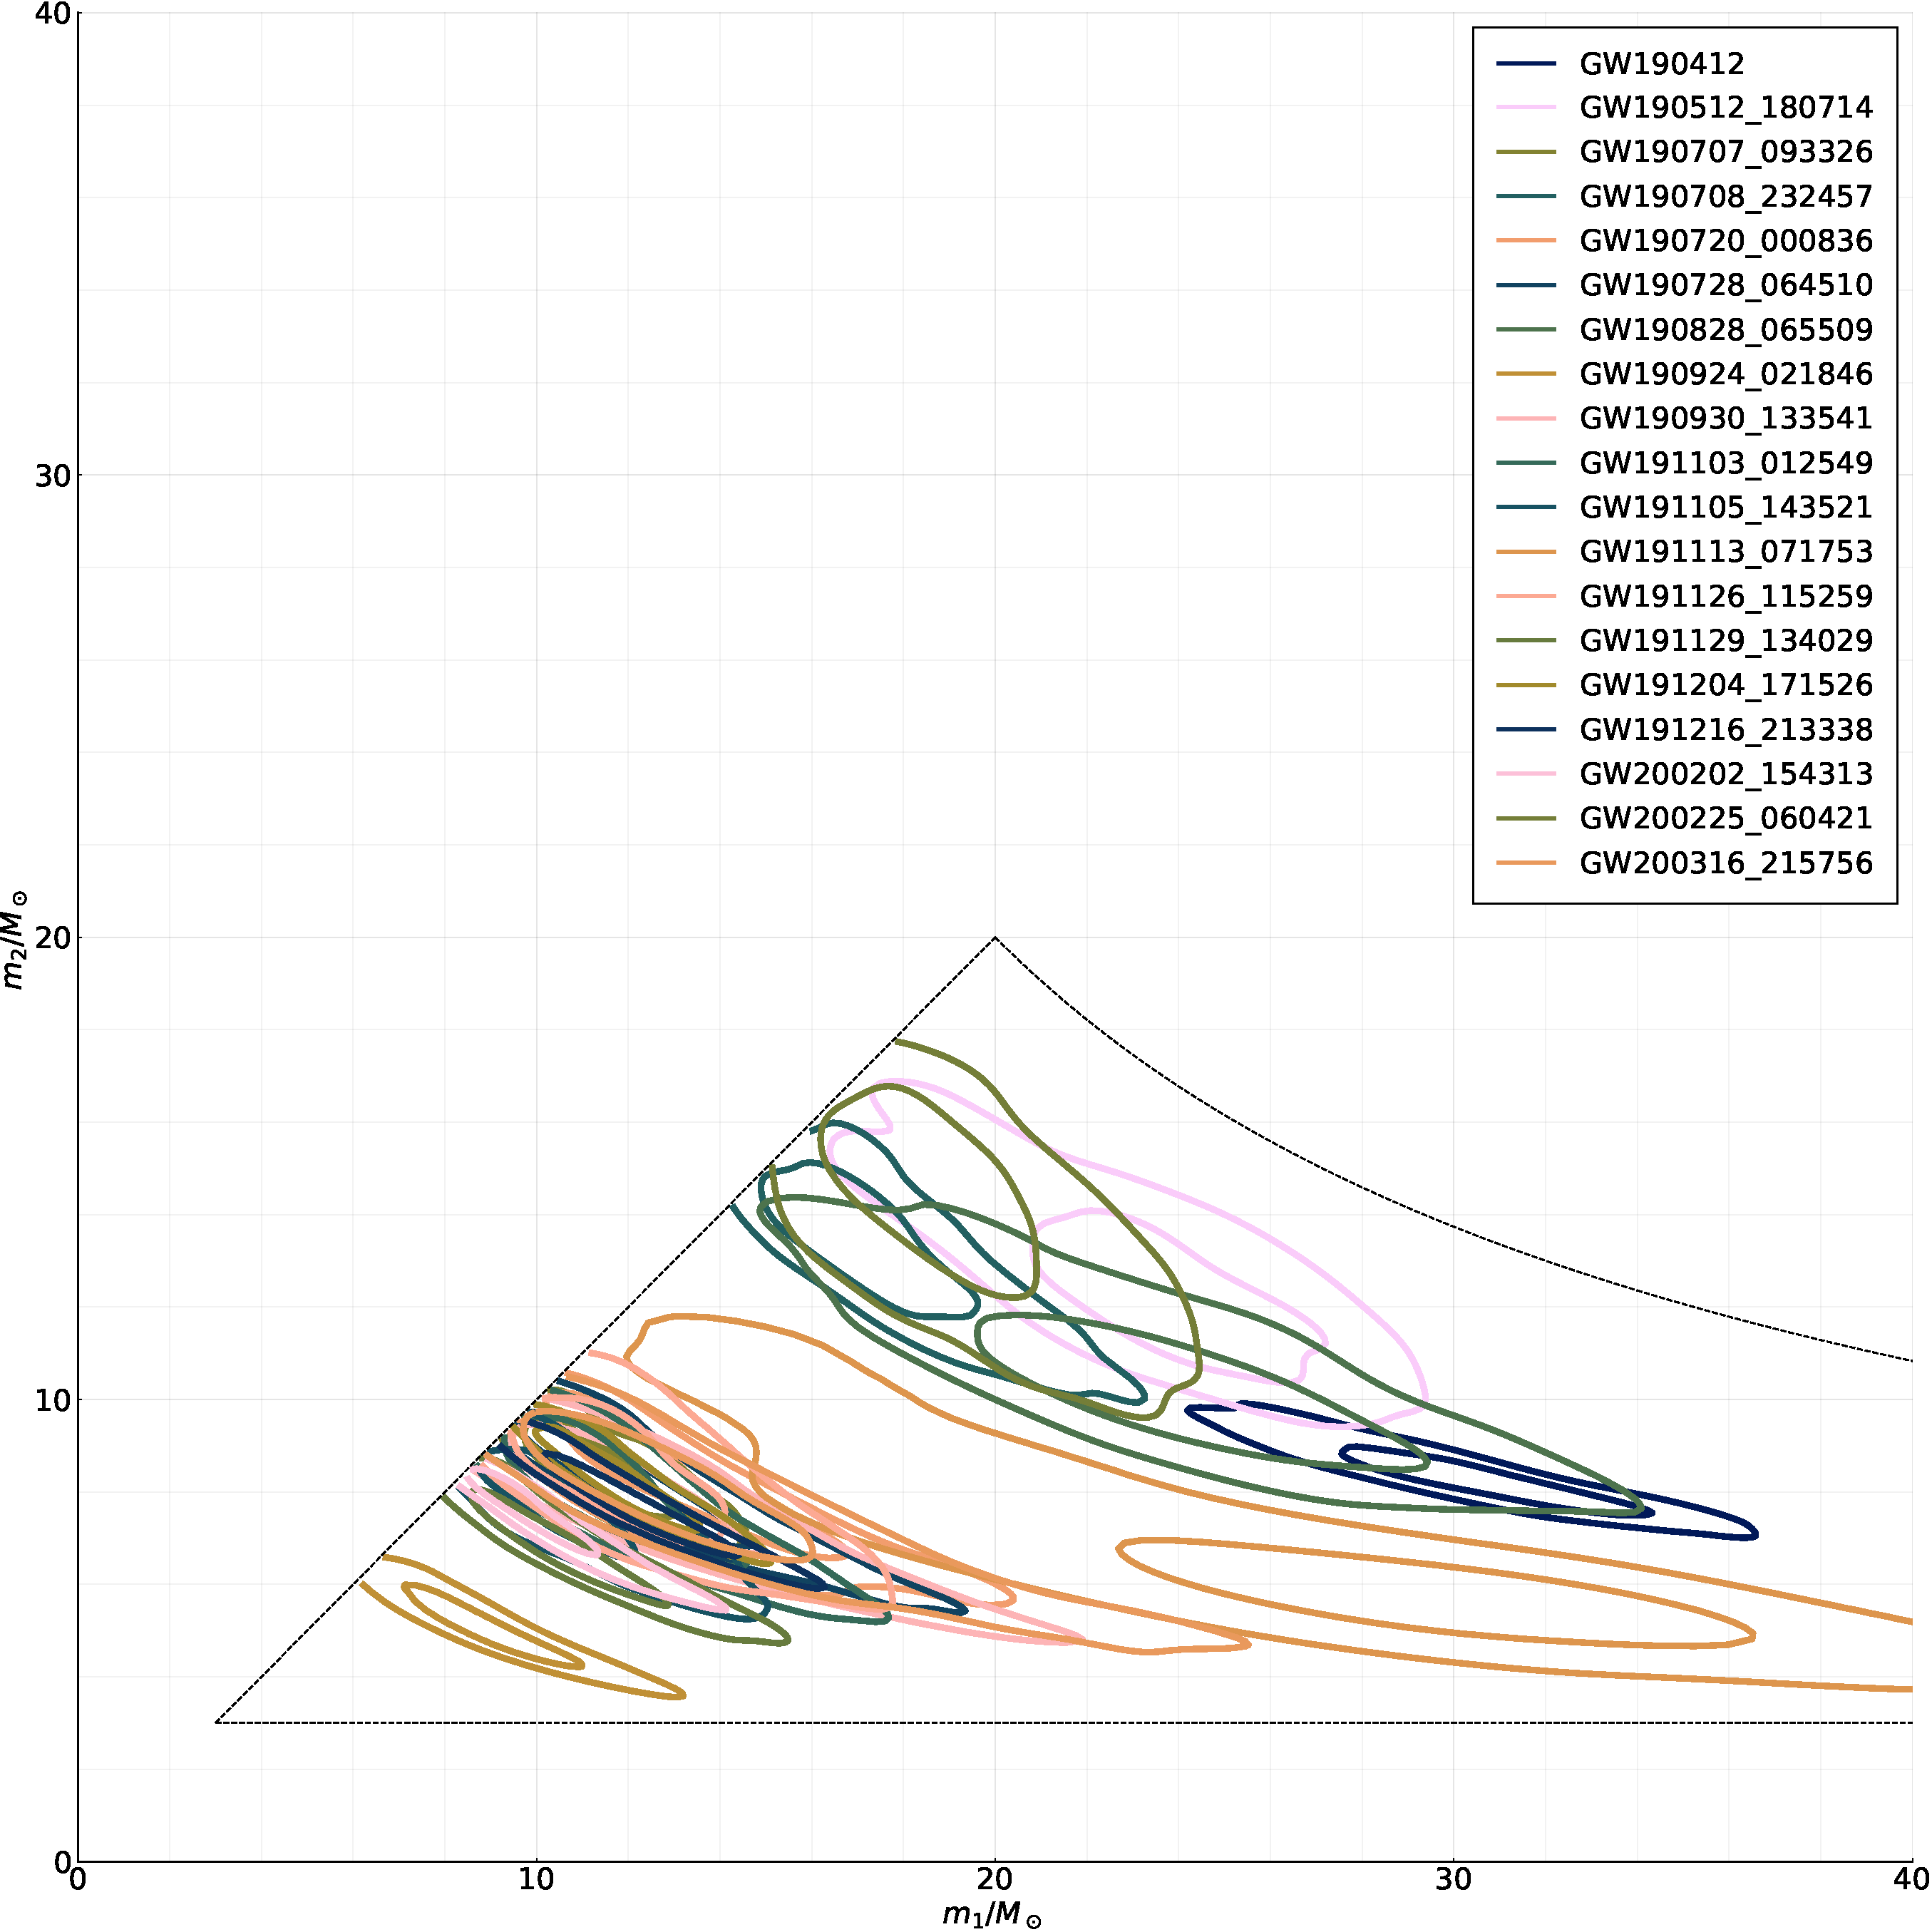
\includegraphics[width=\columnwidth]{figures/m1-m2-contour.pdf}
    \caption{\label{fig:m1-m2-contour} Contour plot of the likelihood functions
    for the primary and secondary black hole masses in the events considered in
    this analysis.  The contours show credible regions containing $50\%$ and
    $90\%$ of the likelihood for each event.  The dashed lines show our
    selection cuts, with $m_1 > 3 \, M_\odot$ and $M_c <
    \mchighunits$.}
\end{figure}

\begin{figure}
    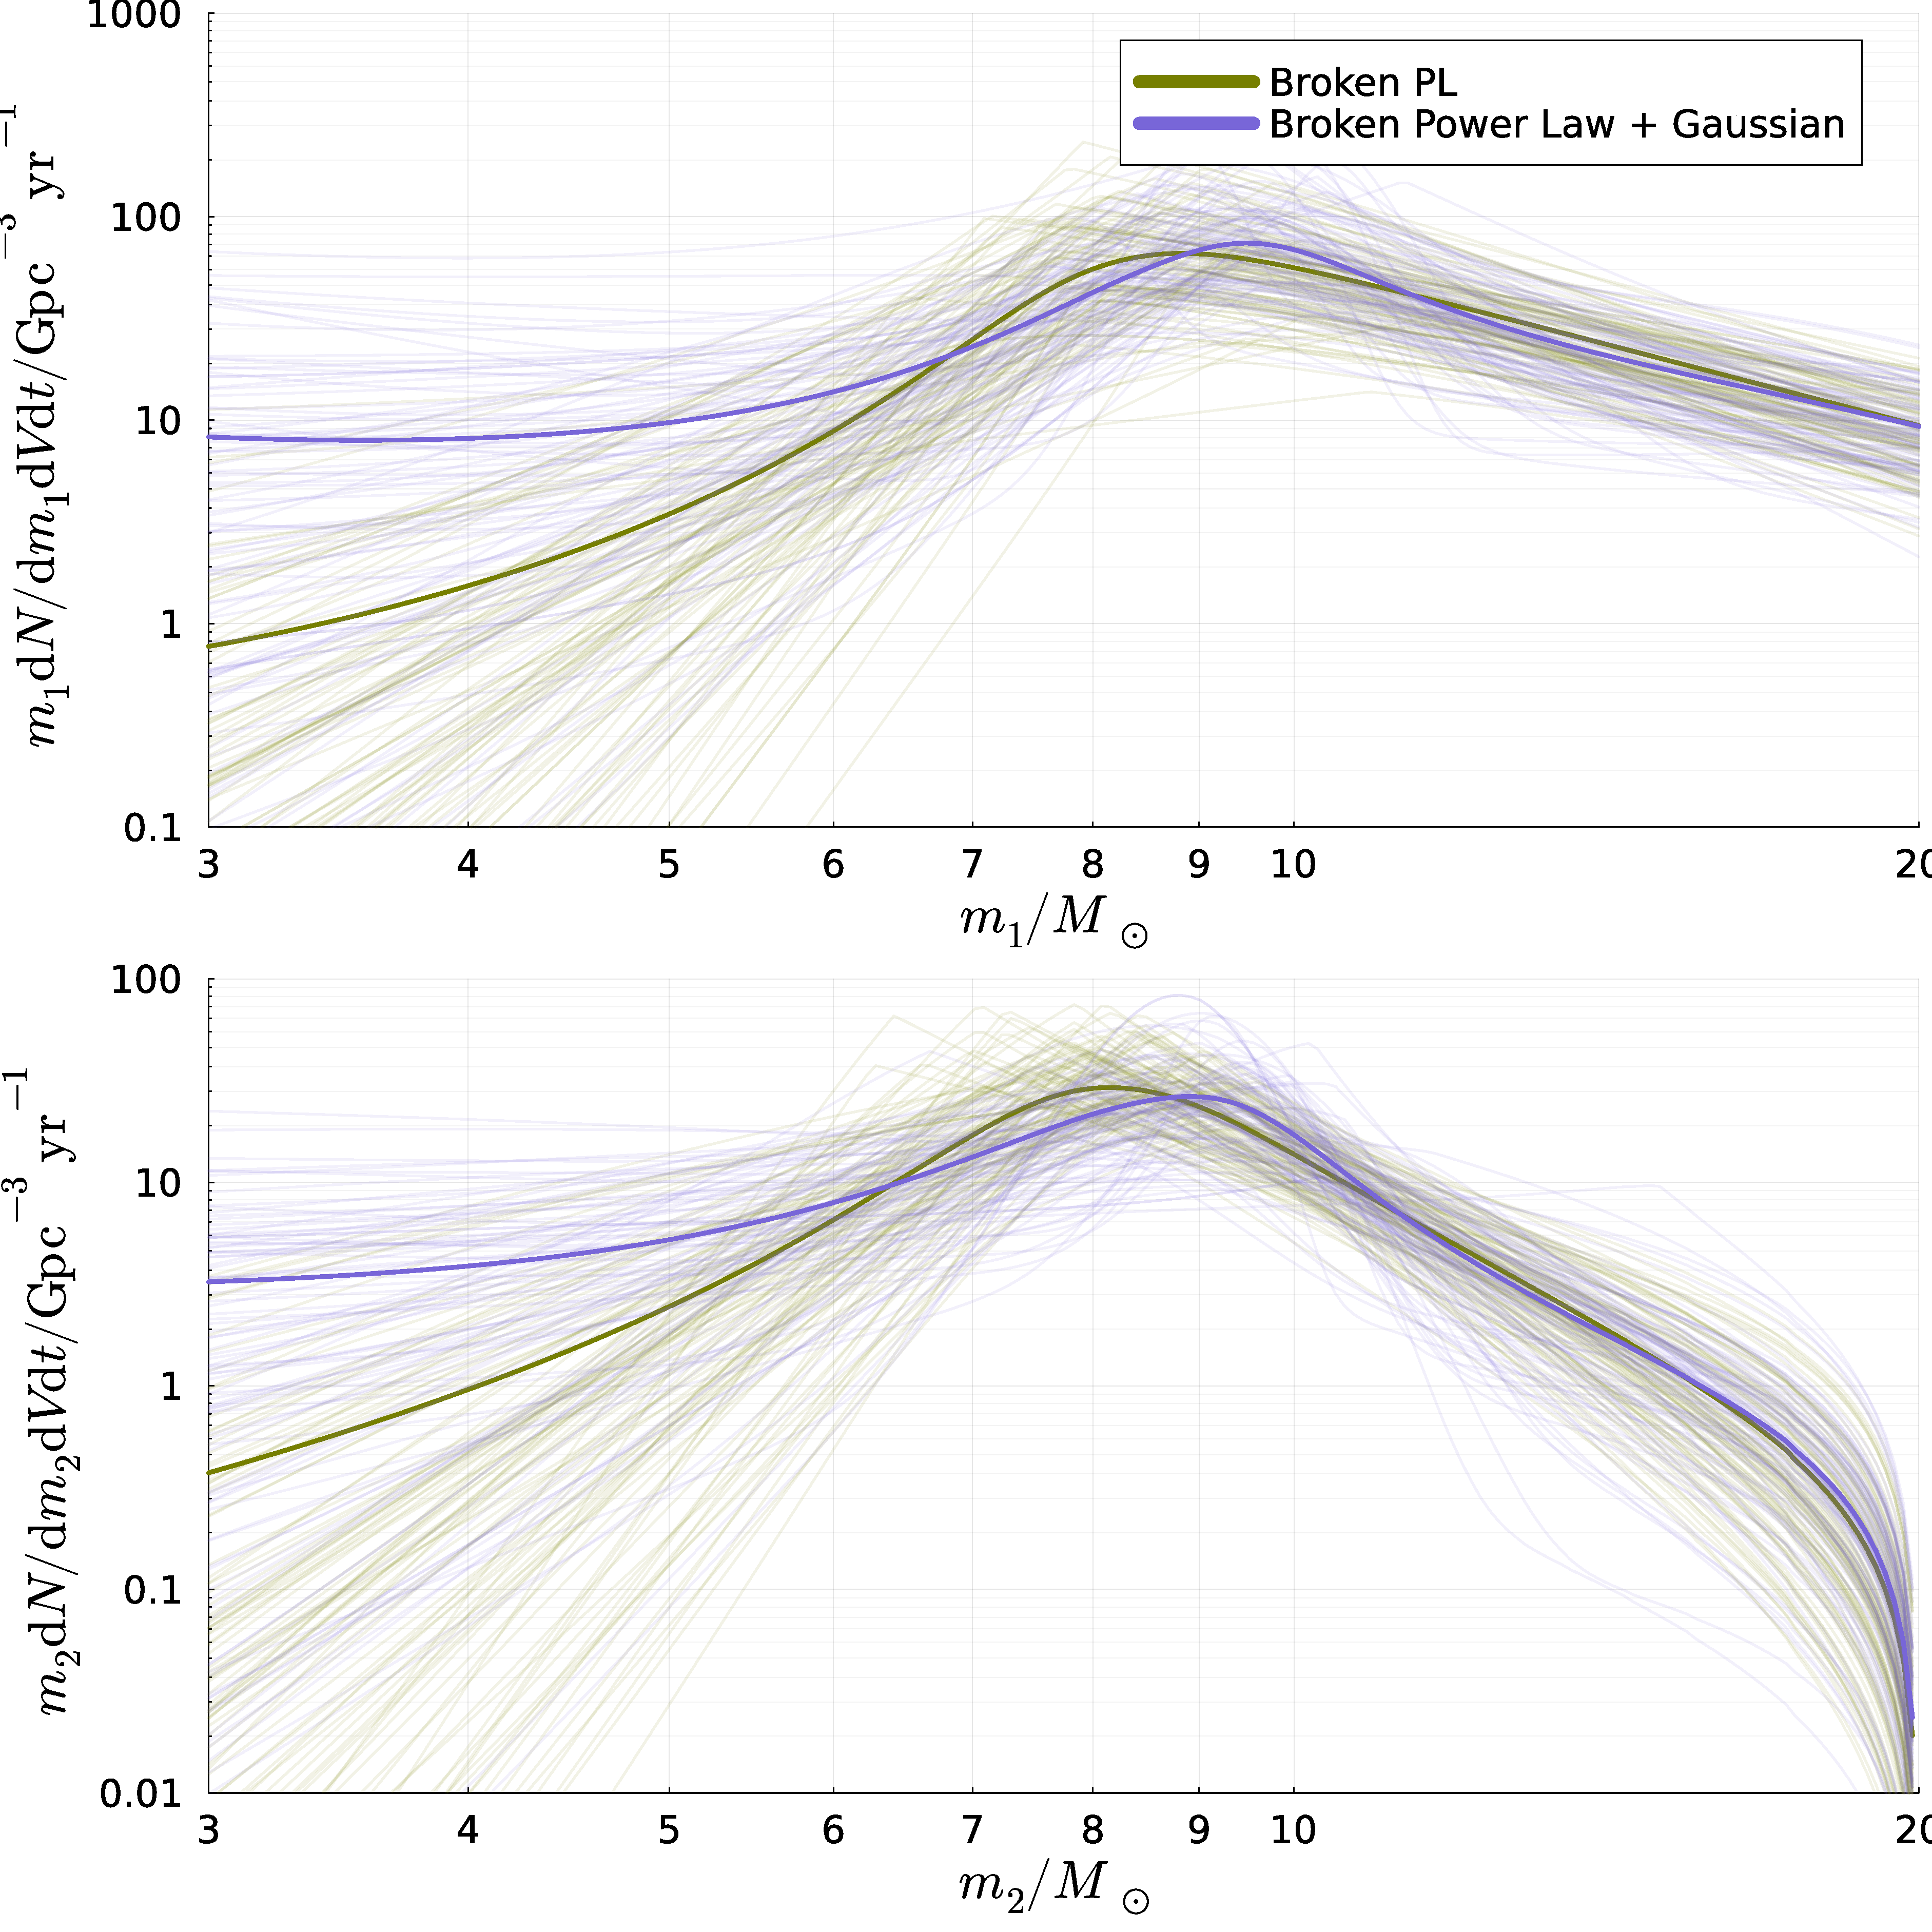
\includegraphics[width=\columnwidth]{figures/dNdm_traces.pdf}
    \caption{\label{fig:dNdm-traces} Inferred mass functions for $3 \, M_\odot <
    m_2 < m_1 < 20 \, M_\odot$ from two models; both primary and secodary
    (marginal) mass functions are shown.  Dark lines show the posterior mean
    mass function; light lines are individual draws from the posterior over mass
    functions.}
\end{figure}

\begin{figure}
    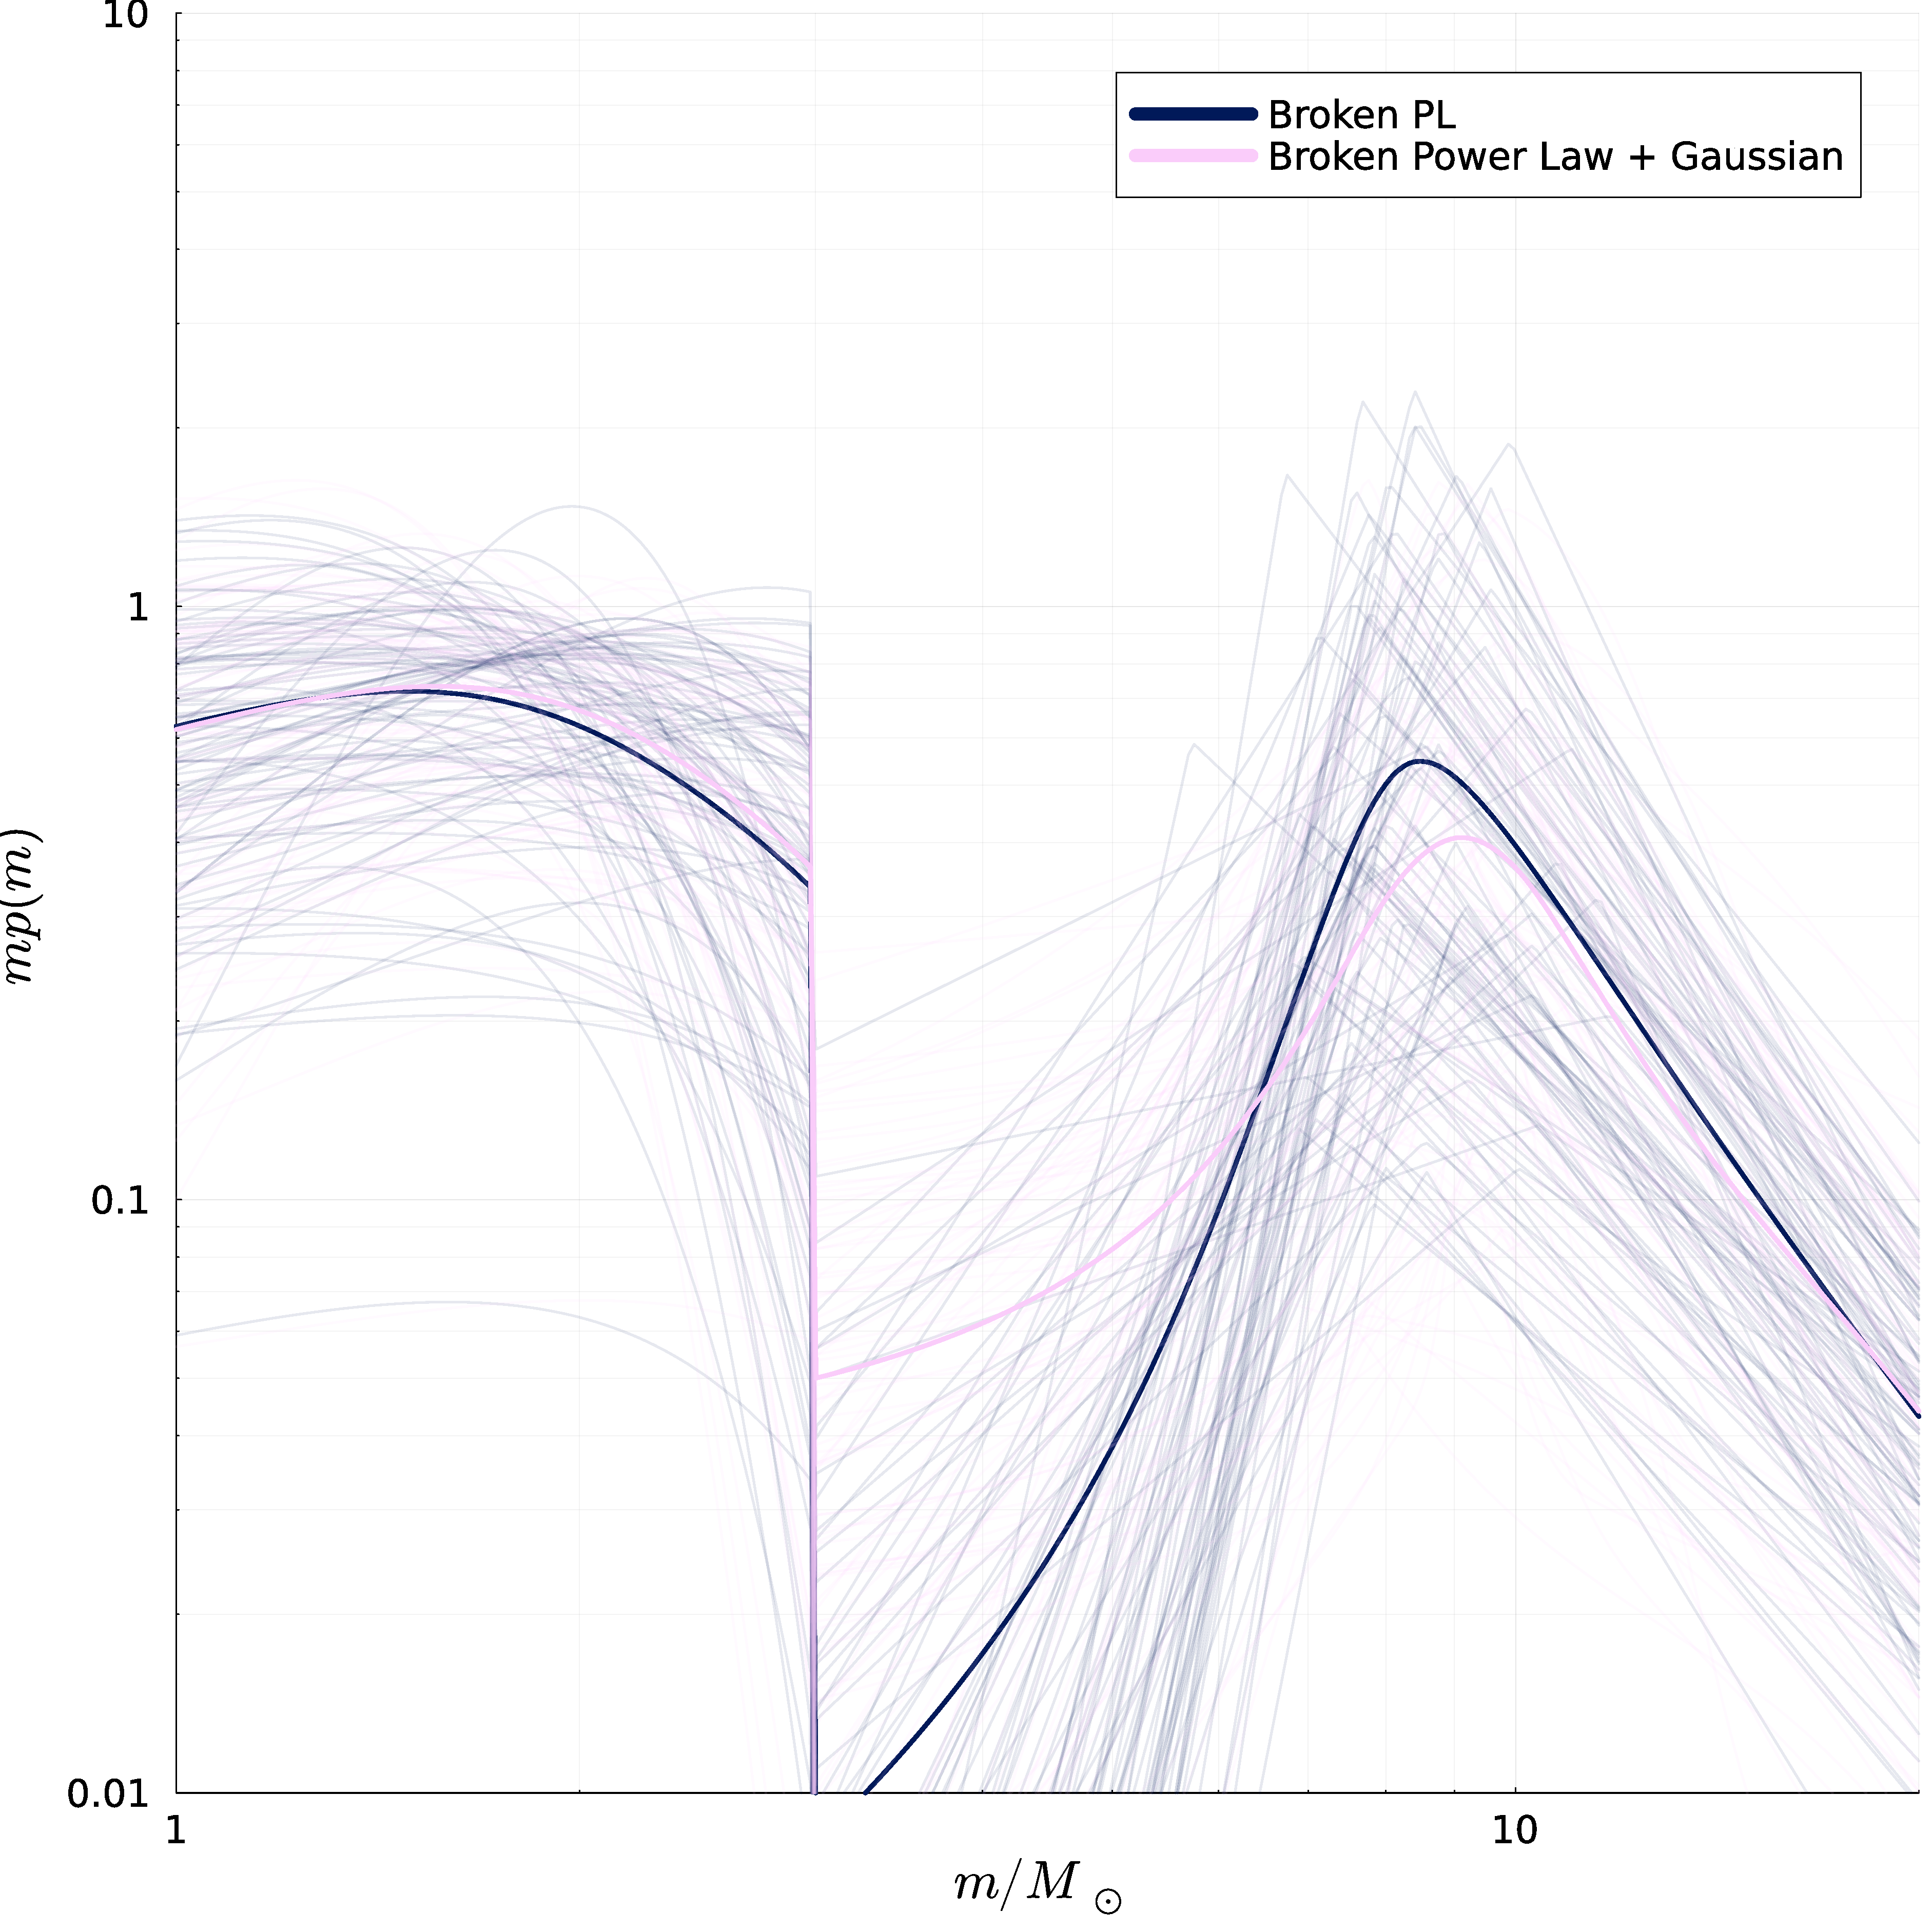
\includegraphics[width=\columnwidth]{figures/pm_traces.pdf}
    \caption{\label{fig:pm-traces} Inferred common mass distribution, $p(m)$,
    (see Eq.~\eqref{eq:pm-definition}) for both models considered in this
    analysis.  Dark lines show the posterior mean mass distribution; light lines
    are individual draws from the posterior over mass distributions.  At high
    masses, $m \gg \mu, m_b$, the mass function falls steeply in both models;
    the broken power law plus Gaussian slope $\alpha_2 = \alphatwoplgplp$.
    Toward lower masses from the peak, both power law models initially decline
    significantly, though the power law plus Gaussian model rises again as $m
    \to 3 \, M_\odot$.}
\end{figure}

\begin{figure}
    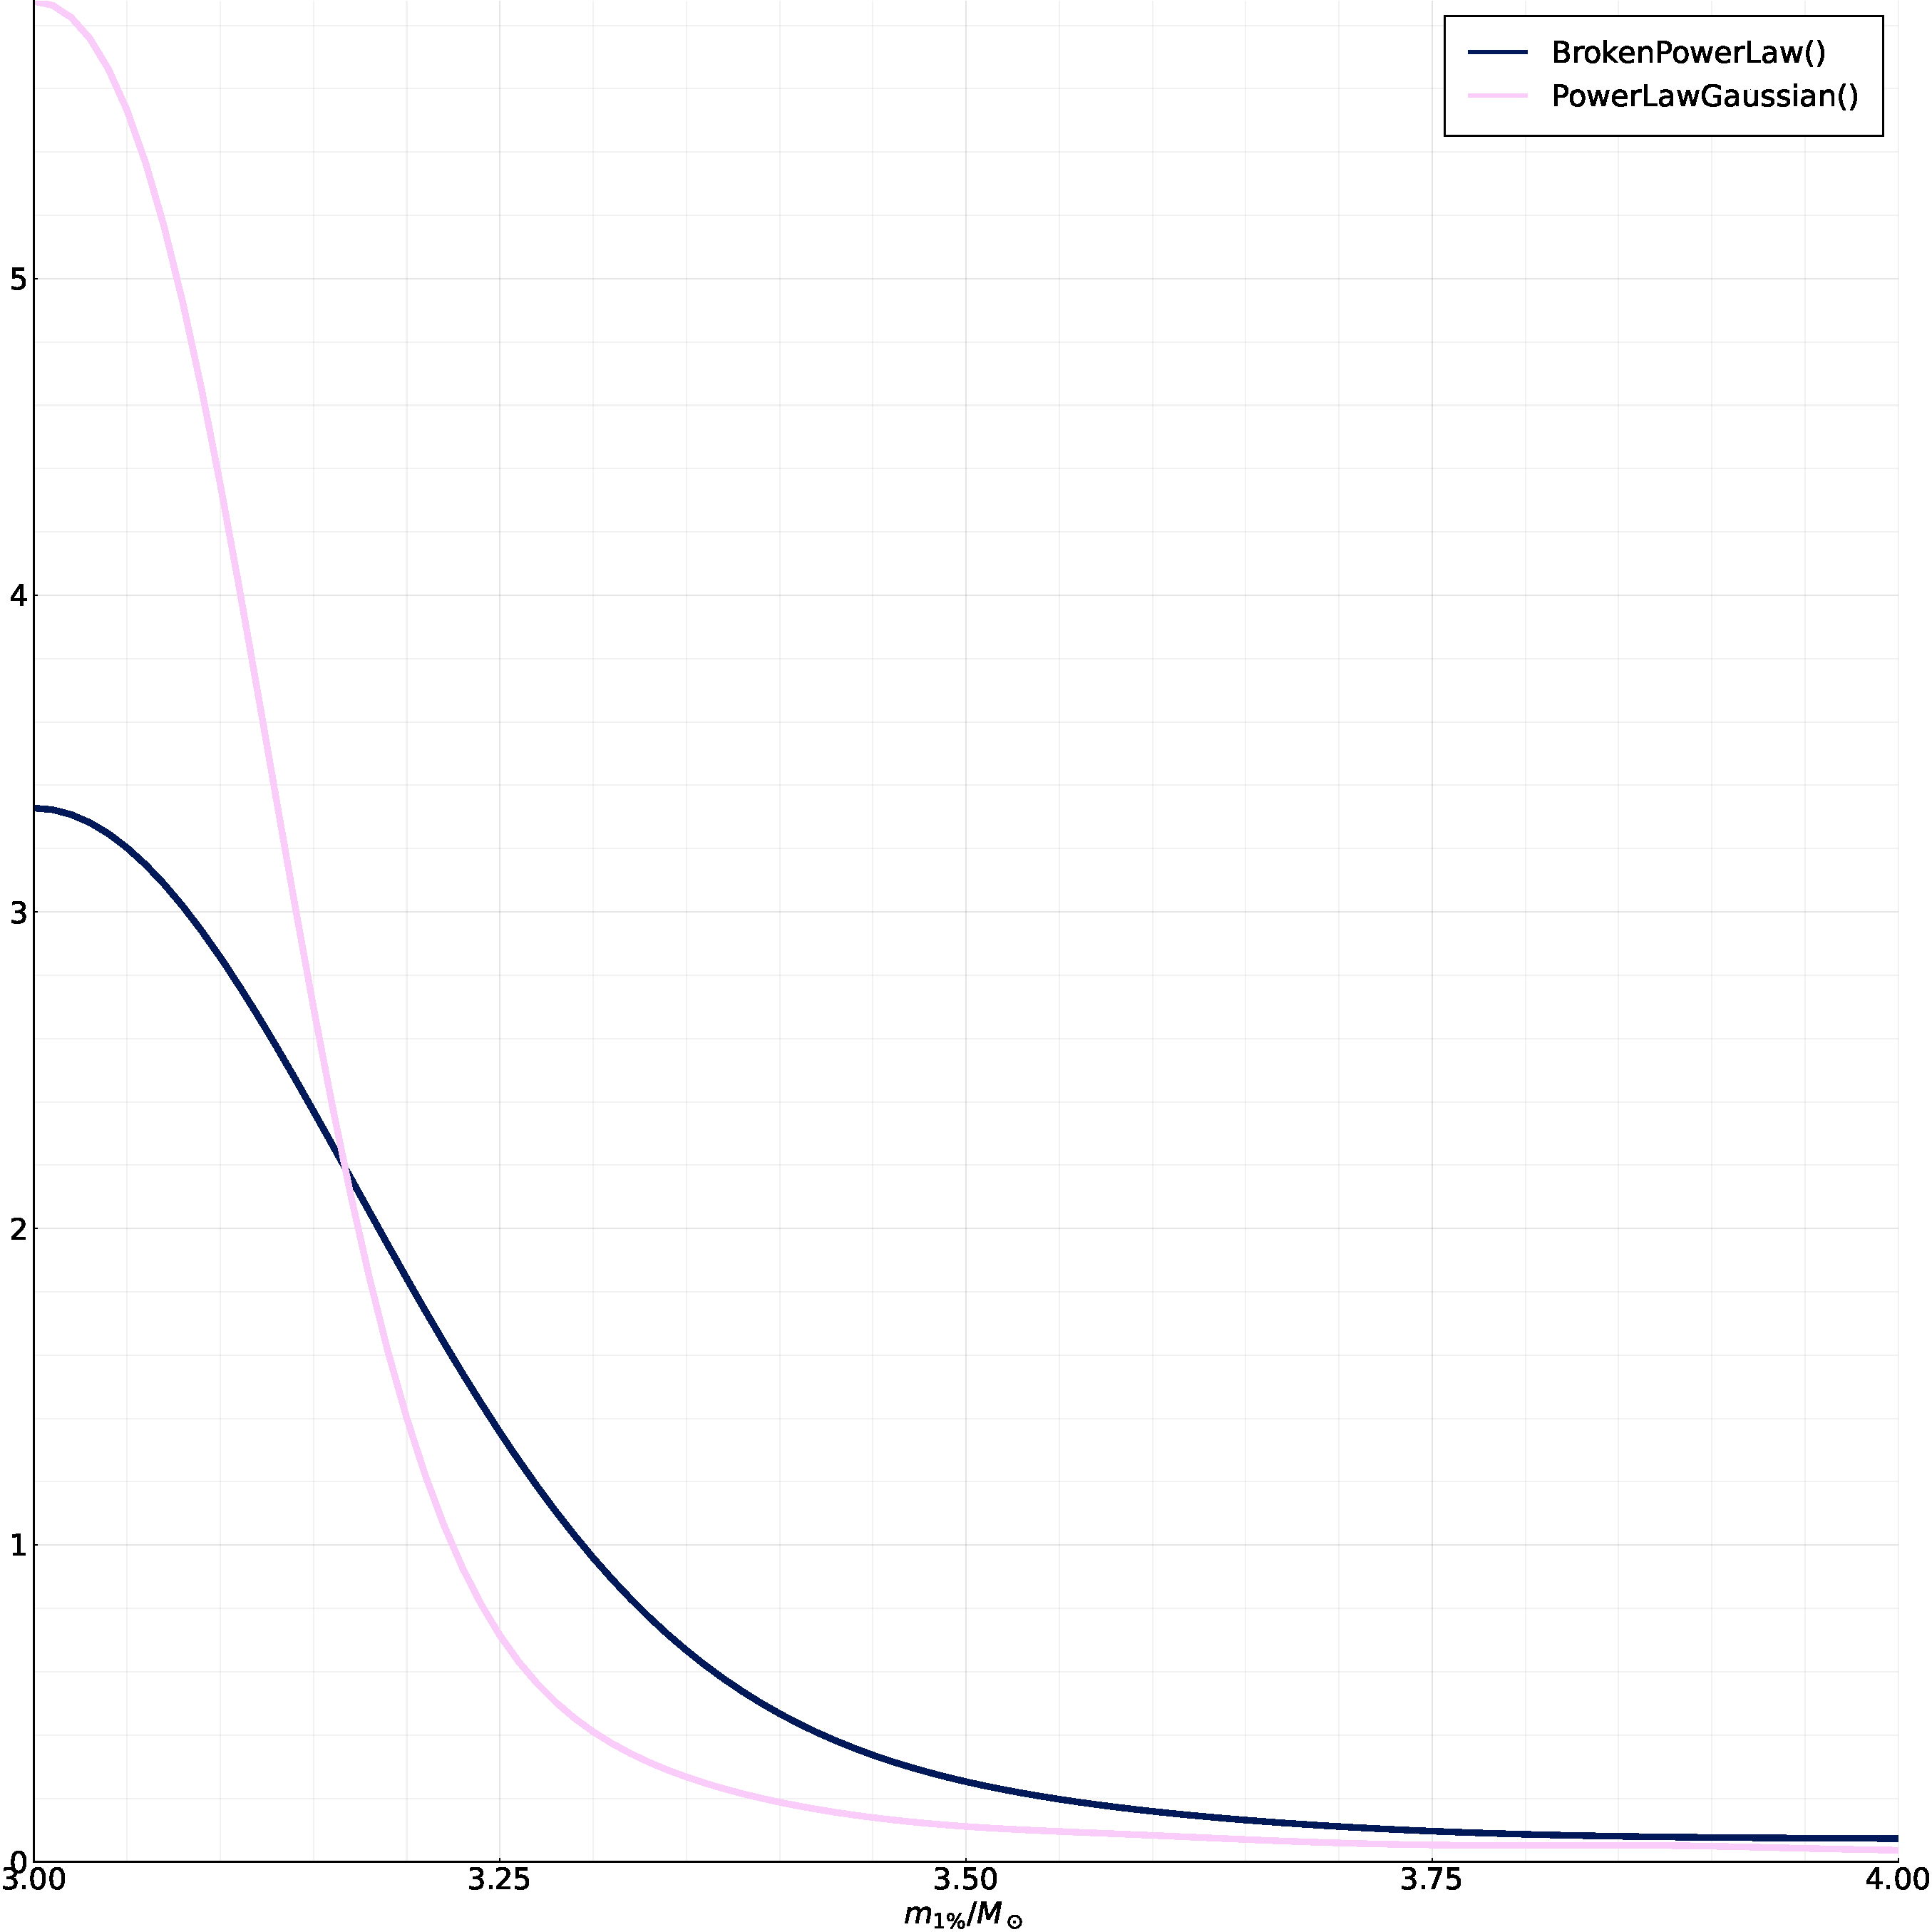
\includegraphics[width=\columnwidth]{figures/m1pct.pdf}
    \caption{\label{fig:m1pct} The posterior distribution for $m_{1\%}$, the
    first percentile of the ``common'' mass function for our three models.  The
    broken power law plus Gaussian model with 50\% selection cut has $m_{1\%} =
    \monepctplgplpunits$ at $1\sigma$ (68\%) credibility.  The solid lines are
    the result for the 50\% selection cut, dashed for the 90\% selection cut.}
\end{figure}

\begin{deluxetable}{llll}
\tablecolumns{3}
\tablecaption{\label{tab:monepct} $m_{1\%}$ for our various models and using different selection functions.}
\tablehead{\colhead{Mass Function Model} & \colhead{$m_{1\%} / M_\odot$ (1-$\sigma$, 68\%)} & \colhead{$m_{1\%} / M_\odot$ range (2-$\sigma$, 95\%)}}
\startdata
\texttt{Broken PL}& $4.93^{+1.04}_{-1.36}$& $\left[3.1, 6.6 \right]$\\ 
\texttt{Broken Power Law + Gaussian}& $3.22^{+1.04}_{-0.12}$& $\left[3.1, 5.7 \right]$\\ 
\enddata
\end{deluxetable}


\begin{acknowledgments}
    We thank Jeff Andrews for comments on an early version of this work.
\end{acknowledgments}

\software{\texttt{zenodo-get} \citep{Volgyes2020}}

\clearpage

\bibliography{Bump10MSun}

\end{document}
